% Created 2022-06-14 Tue 19:42
% Intended LaTeX compiler: pdflatex
\documentclass[smaller]{beamer}\usepackage{listings}
\usepackage{color}
\usepackage{amsmath}
\usepackage{array}
\usepackage[T1]{fontenc}
\usepackage{natbib}
\lstset{
keywordstyle=\color{blue},
commentstyle=\color{red},stringstyle=\color[rgb]{0,.5,0},
literate={~}{$\sim$}{1},
basicstyle=\ttfamily\small,
columns=fullflexible,
breaklines=true,
breakatwhitespace=false,
numbers=left,
numberstyle=\ttfamily\tiny\color{gray},
stepnumber=1,
numbersep=10pt,
backgroundcolor=\color{white},
tabsize=4,
keepspaces=true,
showspaces=false,
showstringspaces=false,
xleftmargin=.23in,
frame=single,
basewidth={0.5em,0.4em},
}
\institute{PhD Student, Section of Biostatistics \\ University of Copenhagen}
\usepackage{natbib, dsfont, pgfpages, tikz,amssymb, amsmath,xcolor}
\bibliographystyle{abbrvnat}
% New operators and commands
\newcommand{\Z}{\mathbb{Z}}
\newcommand{\Q}{\mathbb{Q}}
\newcommand{\R}{\mathbb{R}}
\newcommand{\N}{\mathbb{N}}
\newcommand{\C}{\mathbb{C}}
\renewcommand{\S}{\mathbb{S}}
\newcommand{\blank}{\makebox[1ex]{\textbf{$\cdot$}}}
\newcommand\independent{\protect\mathpalette{\protect\independenT}{\perp}}
\def\independenT#1#2{\mathrel{\rlap{$#1#2$}\mkern2mu{#1#2}}}
\renewcommand{\phi}{\varphi}
\renewcommand{\epsilon}{\varepsilon}
\newcommand*\diff{\mathop{}\!\mathrm{d}}
\newcommand{\weakly}{\rightsquigarrow}
\newcommand\smallO{
  \mathchoice
    {{\scriptstyle\mathcal{O}}}% \displaystyle
    {{\scriptstyle\mathcal{O}}}% \textstyle
    {{\scriptscriptstyle\mathcal{O}}}% \scriptstyle
    {\scalebox{.6}{$\scriptscriptstyle\mathcal{O}$}}%\scriptscriptstyle
}
\newcommand{\midd}{\; \middle|\;}
\newcommand{\1}{\mathds{1}}
\usepackage{ifthen} %% Empirical process with default argument
% \newcommand{\G}[1][]{%
%    \ifthenelse{ \equal{#1}{} }
%       {\ensuremath{\mathbb{G}_n}}
%       {\ensuremath{\mathbb{G}_{#1}}}
% }
% New version:
\newcommand{\G}[2][n]{
{\ensuremath{\mathbb{G}_{#1}}{\left[#2\right]}}
}
\DeclareMathOperator*{\argmin}{\arg\!\min}

% New operators for consistent notation
\newcommand{\V}{\mathrm{Var}} % variance
\newcommand{\measure}[1]{\mathrm{{#1}}} % measure
% \newcommand{\measure}[1]{\textnormal{\textbf{{#1}}}} % measure
\newcommand{\m}[1]{\measure{#1}} % measure shortcut
\newcommand{\eqd}{\stackrel{d}{=}} % equality in distribution
\newcommand{\arrow}[1]{\xrightarrow{\; {#1} \;}}
\newcommand{\arrowP}{\xrightarrow{\; \m{P} \;}} % convergence in probability
\newcommand{\leb}{\lambda} % the Lebesgue measure
\newcommand{\T}{\top} % transpose
\newcommand{\KL}{\ensuremath{D_{\mathrm{KL}}}}

\usepackage{xargs}
% Make it easy to change counterfactual notation:
\newcommandx{\cf}[4][3={}, 4={}]{
  % \ifthenelse{ \equal{#4}{} }
  % {{#1^{#2}}(#3)}
  {\ifthenelse{ \equal{#3}{} }
    {{#1^{#2}}_{#4}}
    {{#1^{#2}}_{#4}(#3)}}
}

% Easily change notation:
\DeclareMathOperator{\TT}{\Psi} % target parameter
\newcommand{\lp}{\mathcal{L}_{\P}^2} % shortcut for lp2 space
\newcommand{\empmeas}{\hat{\mathbb{P}}_n} % empirical measure
\DeclareMathOperator{\E}{\mathbb{E}} % expectation
\renewcommand{\P}{\m{P}} % probability
\newcommand{\ic}{\mathrm{IF}} % influence curve
\setbeamertemplate{footline}[frame number]
\beamertemplatenavigationsymbolsempty
\usepackage{appendixnumberbeamer}
\setbeamercolor{gray}{bg=white!90!black}
\setbeamertemplate{itemize items}{$\circ$}

\renewcommand*\familydefault{\sfdefault}
\itemsep2pt
\usepackage[utf8]{inputenc}
\usepackage[T1]{fontenc}
\usepackage{graphicx}
\usepackage{longtable}
\usepackage{wrapfig}
\usepackage{rotating}
\usepackage[normalem]{ulem}
\usepackage{amsmath}
\usepackage{amssymb}
\usepackage{capt-of}
\usepackage{hyperref}
\usetheme{default}
\author{Anders Munch}
\date{\today}
\title{The negative log-likelihood loss and cross-validation with censored data}
\begin{document}

\maketitle
\begin{frame}{Outline}
\tableofcontents
\end{frame}

\section{Model and hyper-parameter selection for survival models}
\label{sec:org750d397}
\begin{frame}[label={sec:org91a6fc6}]{Selecting a model from a collection of candidate models}
\small Consider estimation of the parameter
\begin{equation*}
  \theta(P) := \argmin_{f \in\mathcal{F}} P[L(f, \blank)],
  \quad \text{where} \quad
  P[g] := \int_{\mathcal{O}}g(o) P(\diff o),
\end{equation*}
for some loss function $L \colon \mathcal{F} \times \mathcal{O} \rightarrow \R_+$.
% We approximate $P$ with the empirical measure $\empmeas$, as
% $\empmeas[L(\tilde{\nu}, \blank)] \approx P[L(\tilde{\nu}, \blank)]$.
% % $\nu(\empmeas)\approx\nu(P)$.

\begin{exampleblock}<2->{\normalsize Maximum likelihood estimator (MLE)}
If \(\mathcal{F}\) is a collection of densities on \(\mathcal{O}\) and \(L(f, O) := -\log(f(O))\), then
\(\theta(\empmeas)\) is the MLE for the model \(\mathcal{F}\), where \(\empmeas\) denotes the empirical
measure.
\end{exampleblock}

\begin{exampleblock}<3->{\normalsize Hyper-parameter selection}
For estimation in high-dimensional settings we often introduce a regularization parameter $\lambda$
(e.g., LASSO, kernel smoothing). To select a value for $\lambda$ we would typically split the data
$\mathcal{D}_n = \{O_1, \dots, O_n\}$ randomly in two, $\mathcal{D}_n^1$ and $\mathcal{D}_n^2$, and
calculate
\begin{equation*}
\argmin_{\lambda\in\Lambda} \empmeas^{2}[L(\hat{f}^{1}_{\lambda}, \blank)],
\end{equation*}
where $\empmeas^2$ denotes the empirical measure based on the sample $\mathcal{D}_n^2$, and
$\hat{f}^1_{\lambda}$ denotes an estimator calculated on $\mathcal{D}_n^1$ with regularization
parameter $\lambda$.
\end{exampleblock}
\end{frame}

\begin{frame}[label={sec:org2934a8a}]{A loss function for survival data}
\small

\begin{description}
\item[{\(O = (\tilde T, \Delta, X) \sim P \in \mathcal{P}\)}] Oberved data with \(\mathcal{O} = \R_+
  \times \{0,1\} \times \R^p\).
\item[{\((T, X) \sim Q \in \mathcal{Q}\)}] The distribution \(Q\) (or a feature of it) is of interest.
\end{description}

\vfill

Assuming coarsening at random \citep{gill1997coarsening} we can write
\begin{equation*}
  \mathcal{P} = \{P_{Q, G} : Q \in \mathcal{Q}, G \in \mathcal{G}\},
\end{equation*}
where $\mathcal{G}$ denotes a collection of conditional distributions for the censoring mechanism,
and the likelihood factorizes as
\begin{equation*}
  \ell(P_{Q, G}, O) = \ell_F(Q, O) \cdot \ell_{\mathcal{C}}(G, O),
\end{equation*}
with
\begin{equation*}
  \ell_F(Q, O) := q(\tilde T \mid X)^{\Delta}\bar{Q}(\tilde T \mid X)^{1-\Delta} m(X),
\end{equation*}
where $q$ and $\bar{Q}$ are the conditional density and survivor function, respectively, and $m$ the
marginal distribution of $X$.

\vfill

Natural to use the negative partial log-likelihood \(-\log\ell_F\) as loss function, or even only the
first part concerning the conditional distribution of \(T\) given \(X\).
\end{frame}

\section{The least false model in the presence of censoring}
\label{sec:org1ccc6a0}
\begin{frame}[label={sec:orgc7dccd3}]{Kullback-Leibler divergence and partial likelihoods}
\small Maximum likelihood estimation is connected to minimizing the Kullback-Leibler
divergence and gives an interpretation of the MLE under mis-specified models.
\begin{equation*}
  \KL(P_0 \, || \, P) := P_0
  {\left[
      % p_1/p_2
    \log \frac{p_0}{p}
  \right]},
  \quad \text{where} \quad
  P_0 = p_0 \cdot \mu,   P = p \cdot \mu.
\end{equation*}

\begin{onlyenv}<1>
\color{white}For a partial likelihood we are minimizing
\begin{equation*}
  Q \longmapsto \KL(P_{Q_0,G} \, || \, P_{Q,G}),
  \quad \text{with} \quad Q \in \mathcal{Q}_*.
\end{equation*}
\color{black}

\vfill

\begin{tikzpicture}
  \draw[line width = .2mm] plot [smooth, tension=.8] coordinates { (0,0) (3,2) (6, 1.2) (9,1)};
  \fill (3,2) circle (0.05);
  \fill (2.6,4) circle (0.05);
  \node[] (PP) at (4,.5) {$\mathcal{P}_*$};
  \node[above] (P) at (2.6,4) {$P_0$};
  \node[below] (G) at (3,2) {$P_*$};
  \draw[dashed] (3,2) -- (2.6,4);
\end{tikzpicture}
\end{onlyenv}

\begin{onlyenv}<2>
For a partial likelihood we are minimizing
\begin{equation*}
  Q \longmapsto \KL(P_{Q_0,G} \, || \, P_{Q,G}),
  \quad \text{with} \quad Q \in \mathcal{Q}_*.
\end{equation*}
\color{black}

\vfill

\begin{tikzpicture}
  \draw[line width = .2mm] plot [smooth, tension=.8] coordinates { (0,0) (3,2) (6, 1.2) (9,1)};
  \fill (3,2) circle (0.05);
  \fill (2.6,4) circle (0.05);
  \node[] (PP) at (4,.5) {$\mathcal{Q}_*$};
  \node[above] (P) at (2.6,4) {$P_{Q_0, G}$};
  \node[below] (G) at (3,2) {$Q_*$};
  \draw[dashed] (2.6,4) -- (3,2);
\end{tikzpicture}
\end{onlyenv}

\begin{onlyenv}<3>
For a partial likelihood we are minimizing
\begin{equation*}
  Q \longmapsto \KL(P_{Q_0,G} \, || \, P_{Q,G}),
  \quad \text{with} \quad Q \in \mathcal{Q}_*.
\end{equation*}
\color{black}

\vfill

\begin{tikzpicture}
  \draw[line width = .2mm] plot [smooth, tension=.8] coordinates { (0,0) (3,2) (6, 1.2) (9,1)};
  \node[] (PP) at (4,.5) {$\mathcal{Q}_*$};
  \node[above] (P) at (2.6,4) {$P_{Q_0, G}$};
  \node[above] (P2) at (6.2,3.5) {$P_{Q_0, \tilde{G}}$};
  \node[below] (G) at (3,2) {$Q_*$};
  \node[below] (D) at (6, 1.2) {$\tilde{Q}_*$};
  \draw[dashed] (P2) -- (D);
  \draw[dashed] (2.6,4) -- (3,2);
  \fill (3,2) circle (0.05);
  \fill (2.6,4) circle (0.05);
  \fill (6, 1.2) circle (0.05);
  \fill (6.2,3.5) circle (0.05);
\end{tikzpicture}
\end{onlyenv}
\end{frame}

\begin{frame}[label={sec:orgd60bf73}]{Least false model depends on the censoring distribution}
\small For any value \(G \in \mathcal{G}\) we have that \(\KL(P_{Q_0,G} \, || \, P_{Q_0,G}) = 0\), so
the correct model \(Q_0\) is ranked better than any other model independently of \(G \in \mathcal{G}\).
However, if \(Q_0 \not \in \mathcal{Q}_*\) the minimizer might depend on the value of \(G\).\footnote{This is mentioned in \cite{whitney2019comment} and \cite{van2003unicv}, and a similar
phenomenon is well studied for the Cox model
\citep{struthers1986misspecified,hjort1992inference,fine2002comparing}.}

\vfill \pause

For the simple survival case with no baseline covariates, we have the following result stating that
for a mis-specified model \(Q\) we can alway find an alternative model \(\tilde Q\) that is ranked
better under one censoring regime but worse under another.

\vfill


\begin{beamercolorbox}[rounded=true]{gray}
Let $Q_0$ and $G$ be given together with some $Q \not = Q_0$. Then (under
regularity conditions) we can find $\tilde Q$ and $\tilde G$ such
that
\begin{equation*}
  \KL(P_{Q_0, G} \, || \, P_{Q, G}) < \KL(P_{Q_0, G} \, || \, P_{\tilde Q, G}),
\end{equation*}
and
\begin{equation*}
  \KL(P_{Q_0, \tilde G} \, || \, P_{Q, \tilde G}) > \KL(P_{Q_0, \tilde G} \, || \, P_{\tilde Q,
    \tilde G}).
\end{equation*}
\end{beamercolorbox}
\end{frame}

\begin{frame}[label={sec:orgf2c8dd2}]{Sketch of proof}
\small
\begin{itemize}
\item Divide \((0, \tau)\) into \((0, \tau_0)\) and \([\tau_0, \tau)\), where \((0, \tau)\) is the
support of \(T\).
\item Construct \(\tilde Q\) such that it performs better than \(Q\) on \((0,\tau_0)\) but worse on
\((\tau_0, \tau)\) under the censoring regime \(G\).
\item Construct \(\tilde G\) such that observations on \((\tau_0, \tau)\) are less likely than under
\(G\).
\end{itemize}

\pause \vfill Whether the alternative model \(\tilde Q\) can be constructed such that \(\tilde Q \in
\mathcal{Q}_*\) for some model class \(\mathcal{Q}_*\) will depend on the model class and on \(Q_0\) and
\(\mathcal{G}\).
\end{frame}

\begin{frame}[label={sec:org529add1}]{A simple example with mis-specified survival models}
\small Assume the data generating distribution given by
\begin{equation*}
  Q_0 = \text{Weibull}(2,  0.5),
  \quad \text{and} \quad
  G_{\gamma} = \text{Weibull}(2,\gamma),
\end{equation*}
and consider the four candidate models indexed by $\alpha$,
\begin{equation*}
  Q_{\alpha} = \text{Exp}(\alpha),
  \quad \text{with} \quad 
  \alpha \in \{1.3, \,1.5,\, 1.8,\, 2\}.
\end{equation*}

\vfill

\begin{onlyenv}<1>
\begin{center}
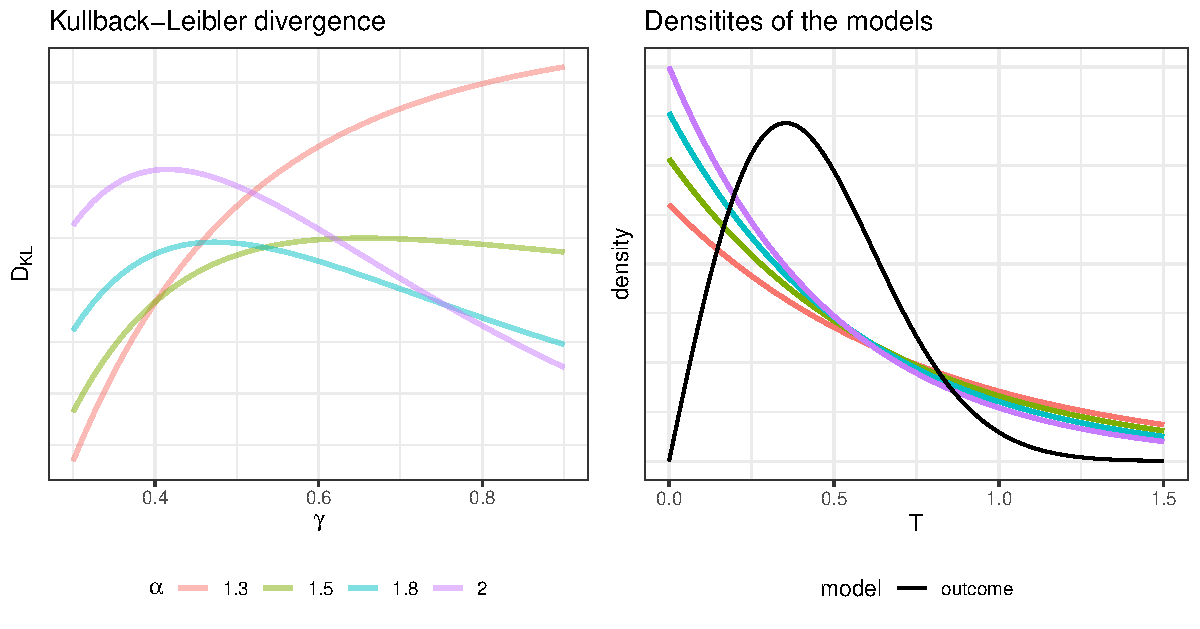
\includegraphics[width=.9\linewidth]{fig-mix-const-v1.pdf}
\end{center}
\end{onlyenv}

\begin{onlyenv}<2>
\begin{center}
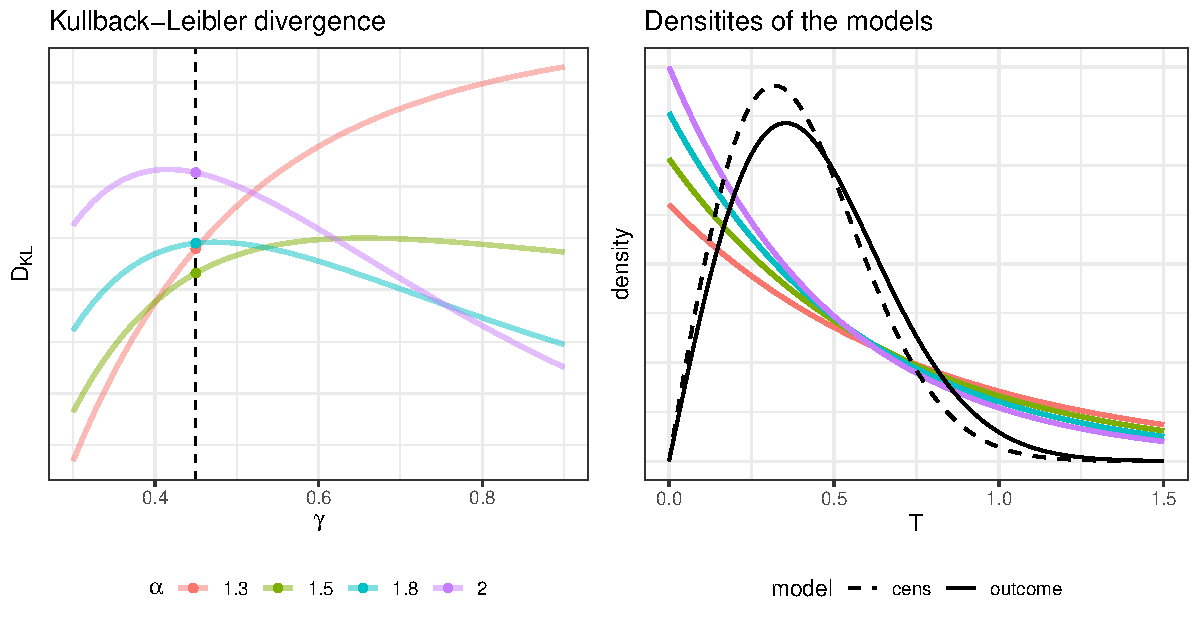
\includegraphics[width=.9\linewidth]{fig-mix-const-v2.pdf}
\end{center}
\end{onlyenv}

\begin{onlyenv}<3>
\begin{center}
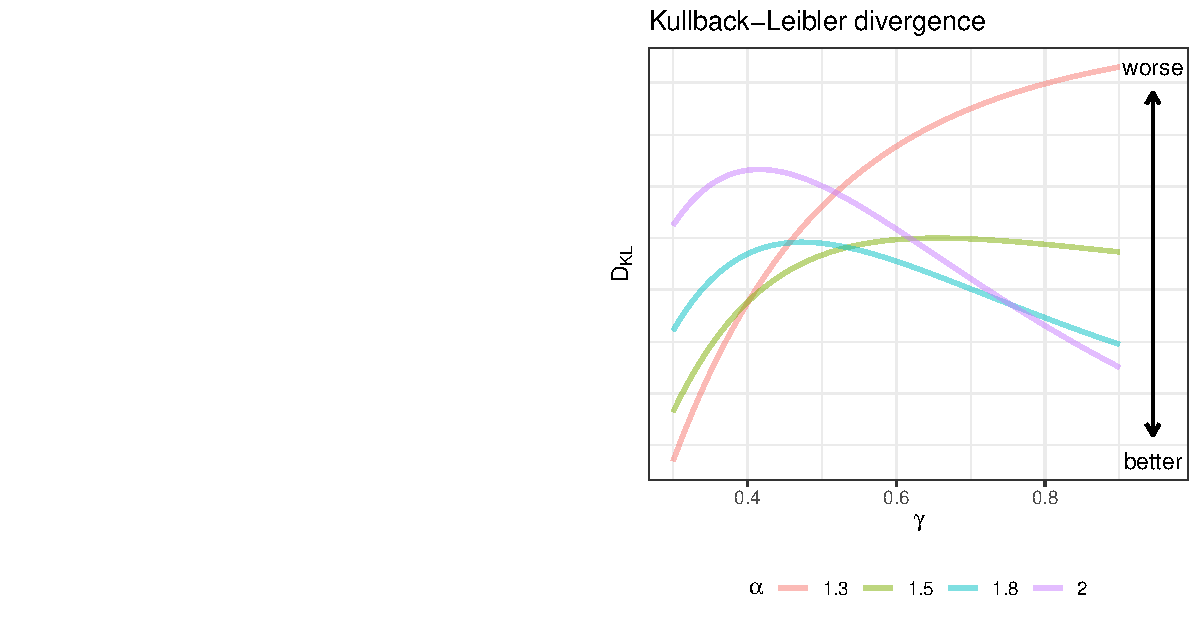
\includegraphics[width=.9\linewidth]{fig-mix-const-v3.pdf}
\end{center}
\end{onlyenv}


\begin{onlyenv}<4>
\begin{center}
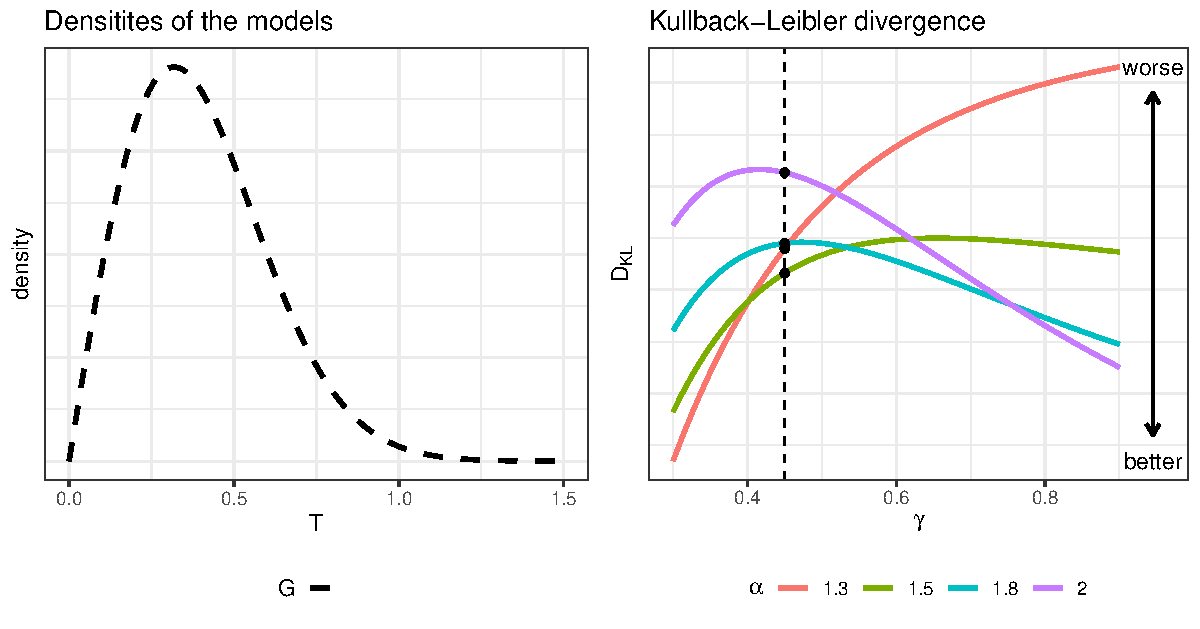
\includegraphics[width=.9\linewidth]{fig-mix-const-v4.pdf}
\end{center}
\end{onlyenv}

\begin{onlyenv}<5>
\begin{center}
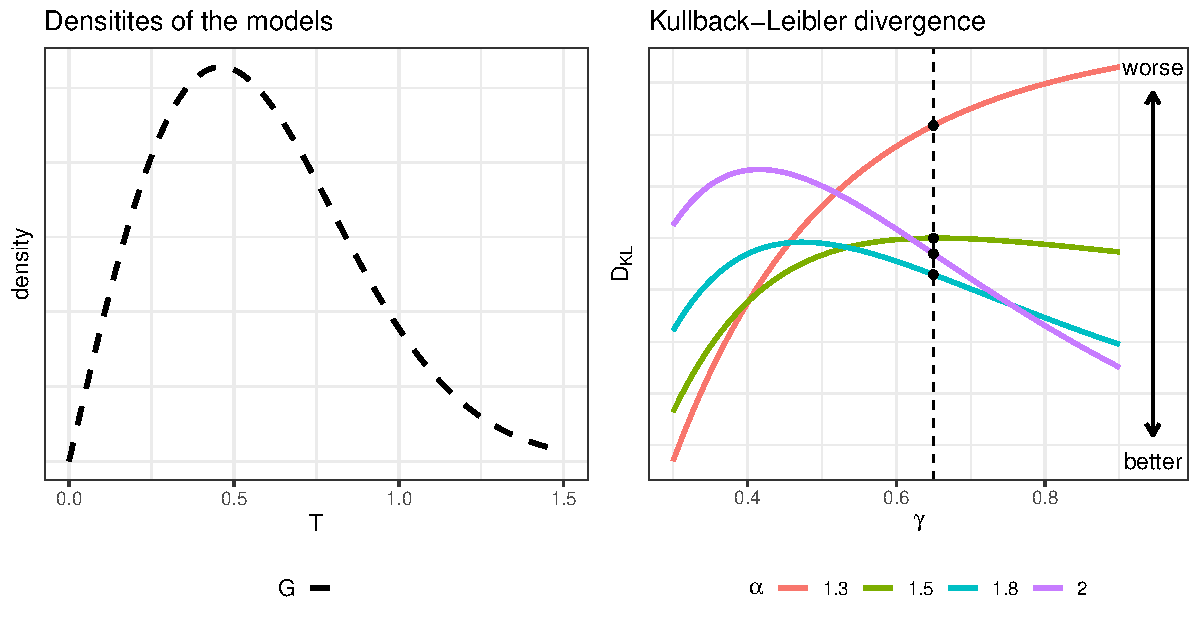
\includegraphics[width=.9\linewidth]{fig-mix-const-v5.pdf}
\end{center}
\end{onlyenv}
\end{frame}

\section{Hold-out samples and survival model estimators}
\label{sec:org500be4f}
\begin{frame}[label={sec:org6bf0f5d}]{Survival curve estimators evaluated on hold-out samples}
\small Consider the problem of selecting a hyper-parameter or model using cross-validation.
We split the data \(\mathcal{D}_n = \{O_1, \dots, O_n\}\) in two, \(\mathcal{D}_n^1\) and \(\mathcal{D}_n^2\).
\begin{description}
\item[{On split \(\mathcal{D}_n^1\)}] Fit models \(\{\hat f_{\lambda} \, : \, \lambda \in \Lambda\}\) or
\(\{\hat f_1, \hat f_2, \dots \hat f_k\}\).
\item[{On split \(\mathcal{D}_n^2\)}] Evalute the performance using a loss function \(L\).
\end{description}

\begin{onlyenv}<1-2>
\pause

\begin{center}
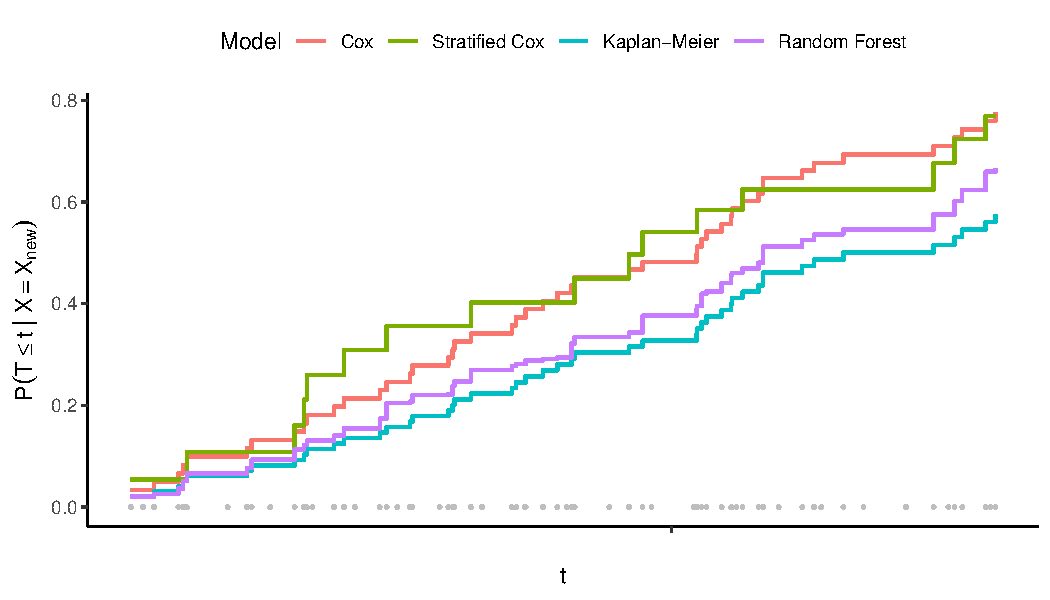
\includegraphics[width=.9\linewidth]{fig-hold-out-sample.pdf}
\end{center}
\end{onlyenv}

\begin{onlyenv}<3>
\begin{center}
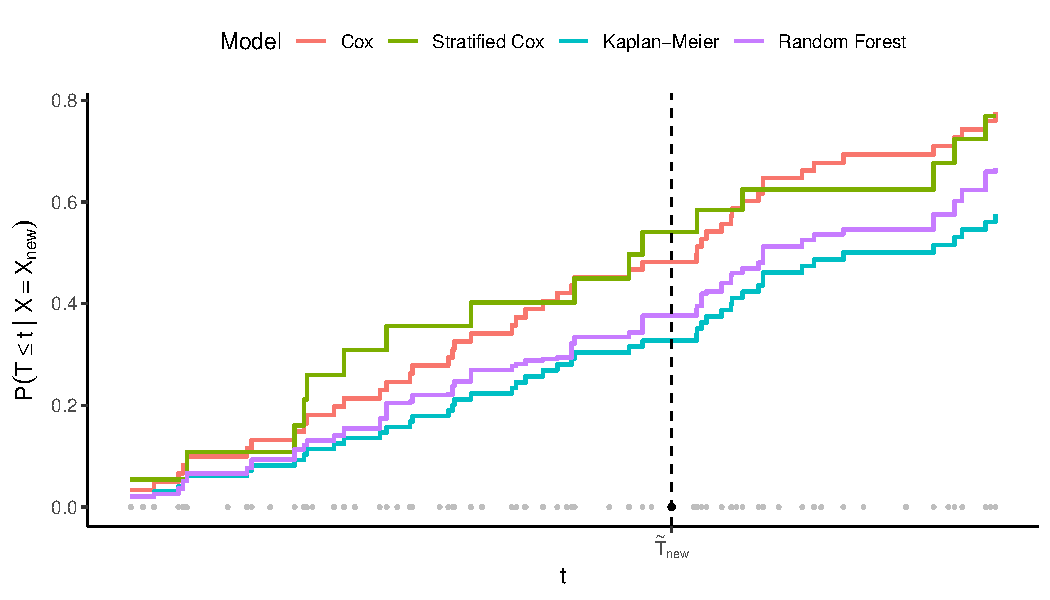
\includegraphics[width=.9\linewidth]{fig-hold-out-sample2.pdf}
\end{center}
\end{onlyenv}
\end{frame}

\begin{frame}[label={sec:org4651003}]{Taking the censoring distribution into account}
\small To alliviate these problems problems we can reweight the observed outcome or the loss
function to account/adjust for the censoring:

\begin{itemize}
\item Inverse probability of censoring weighted loss functions \citep{van2003unicv}. For instance,
weighted negative log-likelihood or (integrated) Brier score.
\item Pseudo-values \citep{andersen2003generalised,mogensen2013random}.
\item Censoring unbiased transformations \citep{fan1996local,steingrimsson2019censoring}.
\end{itemize}

\vfill

These approaches are particularly attractive when we are willing to assume that the censoring does
not depend on the baseline covariates.
\end{frame}

\begin{frame}[label={sec:orgb4592fc}]{Modeling the censoring distribution}
\small If we are not sure that the censoring is independent we need to model the dependence on the
covariates. \vfill


\begin{block}<2->{\centering An (infinite?) loop}
\begin{onlyenv}<1-2>
\pause

\begin{center}
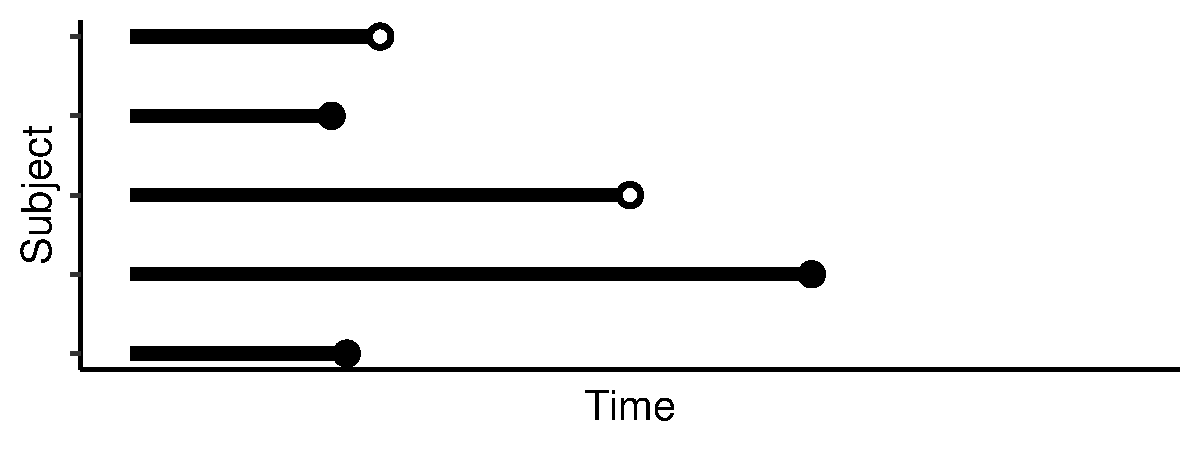
\includegraphics[width=.9\linewidth]{./fig-obs-data.pdf}
\end{center}
\end{onlyenv}

\begin{onlyenv}<3->
\begin{center}
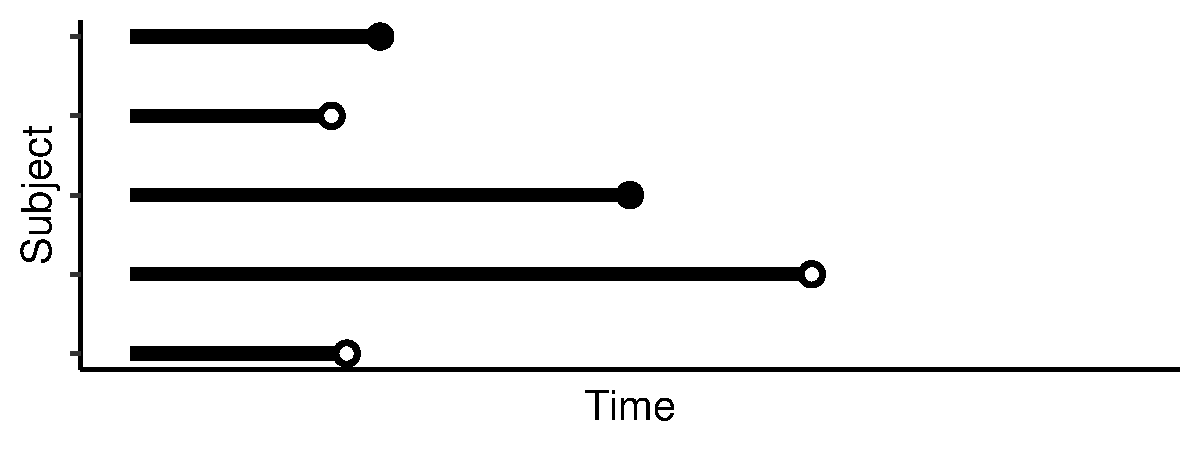
\includegraphics[width=.9\linewidth]{./fig-inverse-data.pdf}
\end{center}
\end{onlyenv}
\end{block}


\begin{onlyenv}<1->
\pause \pause \emph{Inverse-weighted survival games} \citep{han2021inverse}: Iterate the estimation until
convergence (hopefully).
\end{onlyenv}
\end{frame}

\section*{Conclusion}
\label{sec:org33ff113}
\begin{frame}[label={sec:org01bfe2c}]{Conclusion}
\begin{beamercolorbox}[rounded=true]{gray}
\centering How should we do cross-validation for general survival models?
\end{beamercolorbox}

\vfill \small

\begin{itemize}
\item Using the negative partial log-likelihood is problematic
  \begin{itemize}
  \item[$\rightarrow$] The least false model is not well-defined (without reference to the censoring
    regime)
  \item[$\rightarrow$] For many standard survival estimators, we cannot use it on hold-out samples
  \end{itemize}
\item Using loss functions designed to measure the loss for the model of interest is
  challenging in the presence of complicated censoring
  \begin{itemize}
  \item[$\rightarrow$]  We need a model for the censoring ...
    \begin{itemize}
    \item[$\rightarrow$] We need a model for the outcome ...
    \end{itemize}
  \end{itemize}  
\end{itemize}
\vfill \pause

\begin{block}{Questions, comments, suggestions?}
\vfill

\flushright Thank you!
\end{block}
\end{frame}

\section*{References}
\label{sec:orgf065fbb}
\begin{frame}[label={sec:org0fb4580}]{References}
\scriptsize \bibliography{./latex-settings/default-bib.bib}
\end{frame}
\end{document}